\fancyhead[LE,RO]{\textbf{\textsf{34}}\quad \textbf{\textsf{CHƯƠNG 1}}\quad \textsf{Hàm số và Mô hình}}
\fancyhead[RE,LO]{}

\noindent
\begin{minipage}[t]{0.485\textwidth}
\fontsize{8.8pt}{11.2pt}\selectfont
\begin{enumerate}[label=\textbf{\arabic*.}, start=16, itemsep=6pt, parsep=0pt, topsep=1pt, leftmargin=1.4em]
    \item Người quản lý một khu chợ trời cuối tuần biết từ kinh nghiệm trước đây rằng nếu ông tính giá thuê một gian hàng tại chợ là $x$ đô la, thì số lượng gian hàng $y$ được thuê sẽ cho bởi phương trình $y = 200 - 4x$.
    \begin{enumerate}[label=\textbf{(\alph*)}, itemsep=1.5pt, topsep=1.5pt, leftmargin=*]
        \item Hãy phác thảo đồ thị của hàm tuyến tính này. (Lưu ý rằng giá thuê mỗi gian hàng và số lượng gian hàng được thuê không thể là các đại lượng âm.)
        \item Hệ số góc, giao điểm với trục tung ($y$-intercept) và giao điểm với trục hoành ($x$-intercept) của đồ thị biểu thị điều gì?
    \end{enumerate}

    \item Mối liên hệ giữa thang nhiệt độ Fahrenheit ($F$) và Celsius ($C$) được cho bởi hàm tuyến tính $F = \frac{9}{5}C + 32$.
    \begin{enumerate}[label=\textbf{(\alph*)}, itemsep=1.5pt, topsep=1.5pt, leftmargin=*]
        \item Phác thảo đồ thị của hàm số này.
        \item Hệ số góc của đồ thị là bao nhiêu và nó biểu thị điều gì? Giao điểm với trục $F$ ($F$-intercept) là bao nhiêu và nó biểu thị điều gì?
    \end{enumerate}

    \item Jade và bạn cùng phòng Jari đi làm mỗi sáng, di chuyển về phía tây trên đường cao tốc I-10. Vào một buổi sáng, Jade đi làm lúc 6:50 sáng, nhưng Jari khởi hành muộn hơn 10 phút. Cả hai đều lái xe với tốc độ không đổi. Các đồ thị bên dưới cho biết quãng đường (tính bằng dặm) mà mỗi người đã đi được trên đường I-10 sau $t$ phút kể từ 7:00 sáng.
    \begin{enumerate}[label=\textbf{(\alph*)}, itemsep=1.5pt, topsep=1.5pt, leftmargin=*]
        \item Sử dụng đồ thị để xác định ai lái xe nhanh hơn.
        \item Tìm tốc độ (tính theo dặm/giờ, mi/h) của mỗi người.
        \item Tìm các hàm tuyến tính $f$ và $g$ mô hình hóa quãng đường đã đi của Jade và Jari theo biến thời gian $t$ (tính bằng phút).
    \end{enumerate}
    
    \begin{center}
        \vspace{-2pt}
        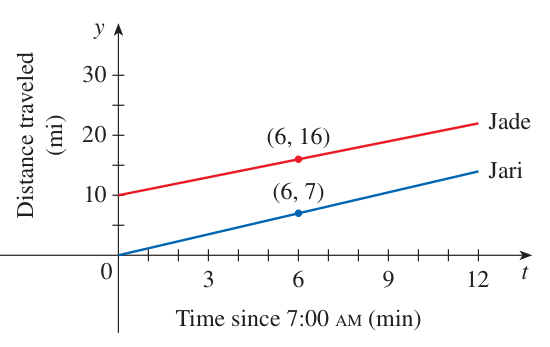
\includegraphics[width=0.76\linewidth]{images/p0069_fig1.png}
        \vspace{-4pt}
    \end{center}

    \item Quản lý của một xưởng sản xuất đồ nội thất nhận thấy chi phí để sản xuất 100 chiếc ghế trong một ngày là \$2200 và chi phí để sản xuất 300 chiếc ghế trong một ngày là \$4800.
    \begin{enumerate}[label=\textbf{(\alph*)}, itemsep=1.5pt, topsep=1.5pt, leftmargin=*]
        \item Biểu diễn chi phí dưới dạng một hàm số theo số lượng ghế được sản xuất, giả sử đây là mối quan hệ tuyến tính. Sau đó vẽ phác thảo đồ thị.
        \item Hệ số góc của đồ thị là bao nhiêu và nó biểu thị điều gì?
        \item Giao điểm với trục tung của đồ thị là bao nhiêu và nó biểu thị điều gì?
    \end{enumerate}

    \item Chi phí hàng tháng để lái một chiếc xe hơi phụ thuộc vào số dặm xe chạy. Lynn nhận thấy rằng trong tháng 5, cô tốn \$380 cho quãng đường 480 dặm và trong tháng 6 tốn \$460 cho 800 dặm.
    \begin{enumerate}[label=\textbf{(\alph*)}, itemsep=1.5pt, topsep=1.5pt, leftmargin=*]
        \item Biểu diễn chi phí hàng tháng $C$ như một hàm số của quãng đường đã đi $d$, giả thiết rằng một mối quan hệ tuyến tính cung cấp mô hình phù hợp.
        \item Sử dụng kết quả phần (a) để dự đoán chi phí khi lái xe 1500 dặm trong một tháng.
        \item Vẽ đồ thị của hàm tuyến tính. Hệ số góc biểu thị điều gì?
        \item Giao điểm với trục $C$ ($C$-intercept) biểu thị điều gì?
        \item Tại sao một hàm tuyến tính lại cung cấp một mô hình phù hợp trong tình huống này?
    \end{enumerate}
\end{enumerate}
\end{minipage}%
\hfill
\begin{minipage}[t]{0.485\textwidth}
\fontsize{8.8pt}{11.2pt}\selectfont
\begin{enumerate}[label=\textbf{\arabic*.}, start=21, itemsep=6pt, parsep=0pt, topsep=1pt, leftmargin=1.4em]
    \item Tại mặt nước biển, áp suất nước bằng với áp suất khí quyển phía trên mặt nước, là $15\text{ lb/in}^2$. Dưới mặt nước biển, áp suất nước tăng thêm $4{,}34\text{ lb/in}^2$ sau mỗi $10\text{ ft}$ lặn sâu.
    \begin{enumerate}[label=\textbf{(\alph*)}, itemsep=1.5pt, topsep=1.5pt, leftmargin=*]
        \item Biểu diễn áp suất nước dưới dạng một hàm số theo độ sâu phía dưới mặt biển.
        \item Ở độ sâu nào thì áp suất nước đạt $100\text{ lb/in}^2$?
    \end{enumerate}

    \item Điện trở $R$ của một đoạn dây dẫn có chiều dài cố định liên hệ với đường kính $x$ của nó theo định luật tỉ lệ nghịch với bình phương, nghĩa là thông qua một hàm số có dạng $R(x) = kx^{-2}$.
    \begin{enumerate}[label=\textbf{(\alph*)}, itemsep=1.5pt, topsep=1.5pt, leftmargin=*]
        \item Một đoạn dây dẫn có chiều dài cố định và đường kính $0{,}005\text{ m}$ có điện trở $140\,\Omega$. Hãy tìm giá trị của $k$.
        \item Tìm điện trở của một đoạn dây dẫn làm từ cùng vật liệu và có cùng chiều dài như đoạn dây ở câu (a) nhưng có đường kính là $0{,}008\text{ m}$.
    \end{enumerate}

    \item Độ chiếu sáng của một vật bởi một nguồn sáng liên hệ với khoảng cách từ nguồn tới vật theo định luật tỉ lệ nghịch với bình phương. Giả sử sau khi trời tối, bạn đang ngồi đọc sách trong một căn phòng chỉ có một bóng đèn duy nhất. Ánh sáng quá mờ, vì vậy bạn kéo ghế lại gần đèn sao cho khoảng cách giảm đi một nửa. Ánh sáng lúc này sẽ sáng hơn bao nhiêu lần?

    \item Áp suất $P$ của một lượng khí oxy bị nén ở nhiệt độ không đổi liên hệ với thể tích $V$ của chất khí theo hàm tỉ lệ nghịch có dạng $P = k/V$.
    \begin{enumerate}[label=\textbf{(\alph*)}, itemsep=1.5pt, topsep=1.5pt, leftmargin=*]
        \item Một mẫu khí oxy chiếm thể tích $0{,}671\text{ m}^3$ sinh ra áp suất $39\text{ kPa}$ ở nhiệt độ $293\text{ K}$ (nhiệt độ tuyệt đối tính theo thang Kelvin). Hãy tìm giá trị của $k$ trong mô hình đã cho.
        \item Nếu mẫu khí dãn nở đến thể tích $0{,}916\text{ m}^3$, hãy tìm giá trị áp suất mới.
    \end{enumerate}

    \item Công suất đầu ra của tuabin gió phụ thuộc vào nhiều yếu tố. Bằng các nguyên lý vật lý, người ta chứng minh được rằng công suất $P$ do tuabin gió tạo ra được mô hình hóa bởi
    \[
    P = kAv^3
    \]
    trong đó $v$ là tốc độ gió, $A$ là diện tích quét của cánh quạt, và $k$ là một hằng số phụ thuộc vào khối lượng riêng của không khí, hiệu suất của tuabin và thiết kế cánh quạt tuabin.
    \begin{enumerate}[label=\textbf{(\alph*)}, itemsep=1.5pt, topsep=1.5pt, leftmargin=*]
        \item Nếu chỉ có tốc độ gió tăng gấp đôi, thì công suất đầu ra tăng lên theo hệ số bao nhiêu?
        \item Nếu chỉ có chiều dài của cánh quạt tăng gấp đôi, thì công suất đầu ra tăng lên theo hệ số bao nhiêu?
        \item Đối với một tuabin gió cụ thể, chiều dài cánh quạt là $30\text{ m}$ và $k = 0{,}214\text{ kg/m}^3$. Hãy tìm công suất đầu ra (tính bằng watt, $\text{W} = \text{m}^2\cdot\text{kg/s}^3$) khi tốc độ gió lần lượt là $10\text{ m/s}$, $15\text{ m/s}$ và $25\text{ m/s}$.
    \end{enumerate}

    \item Các nhà thiên văn học xác định năng lượng phát xạ toàn phần (thông lượng bức xạ phát ra trên một đơn vị diện tích) của các ngôi sao bằng cách sử dụng Định luật Stefan--Boltzmann:
    \[
    E(T) = (5{,}67 \times 10^{-8})T^4
    \]
    trong đó $E$ là năng lượng bức xạ trên một đơn vị diện tích bề mặt
\end{enumerate}
\end{minipage}